\section{Experimental Environment}
\label{sec:platform}

	\mppa processor is one of the architectures supported by Nanvix and will be
	used as a case study in this work. As Figure~\ref{fig:mppa} pictures,
	\mppa integrates 288 general-purpose cores, grouped into 16 \cclusters,
	intended for useful computing, and 4 \ioclusters responsible for
	communicating with peripherals. On the one hand, each \ccluster integrates
	16~\pes, 1~\rman, 2~MB of local \sram, two \noc interfaces, and does not
	have hardware support for cache coherence. On the other hand, each
	\iocluster features 4\rmans, 4~MB of \sram, and 8 \noc interfaces. Two of
	these \ioclusters have access to a 4~GB of \dram, and the other two are
	connected to Ethernet controllers. Two distinct 2-D Torus \nocs handle
	inter-cluster communication. Specifically, \cnoc allows the exchanging of
	small control messages, and \dnoc supports the transferring of arbitrary
	amounts of data.

	\begin{figure}[tb]
			\centering
			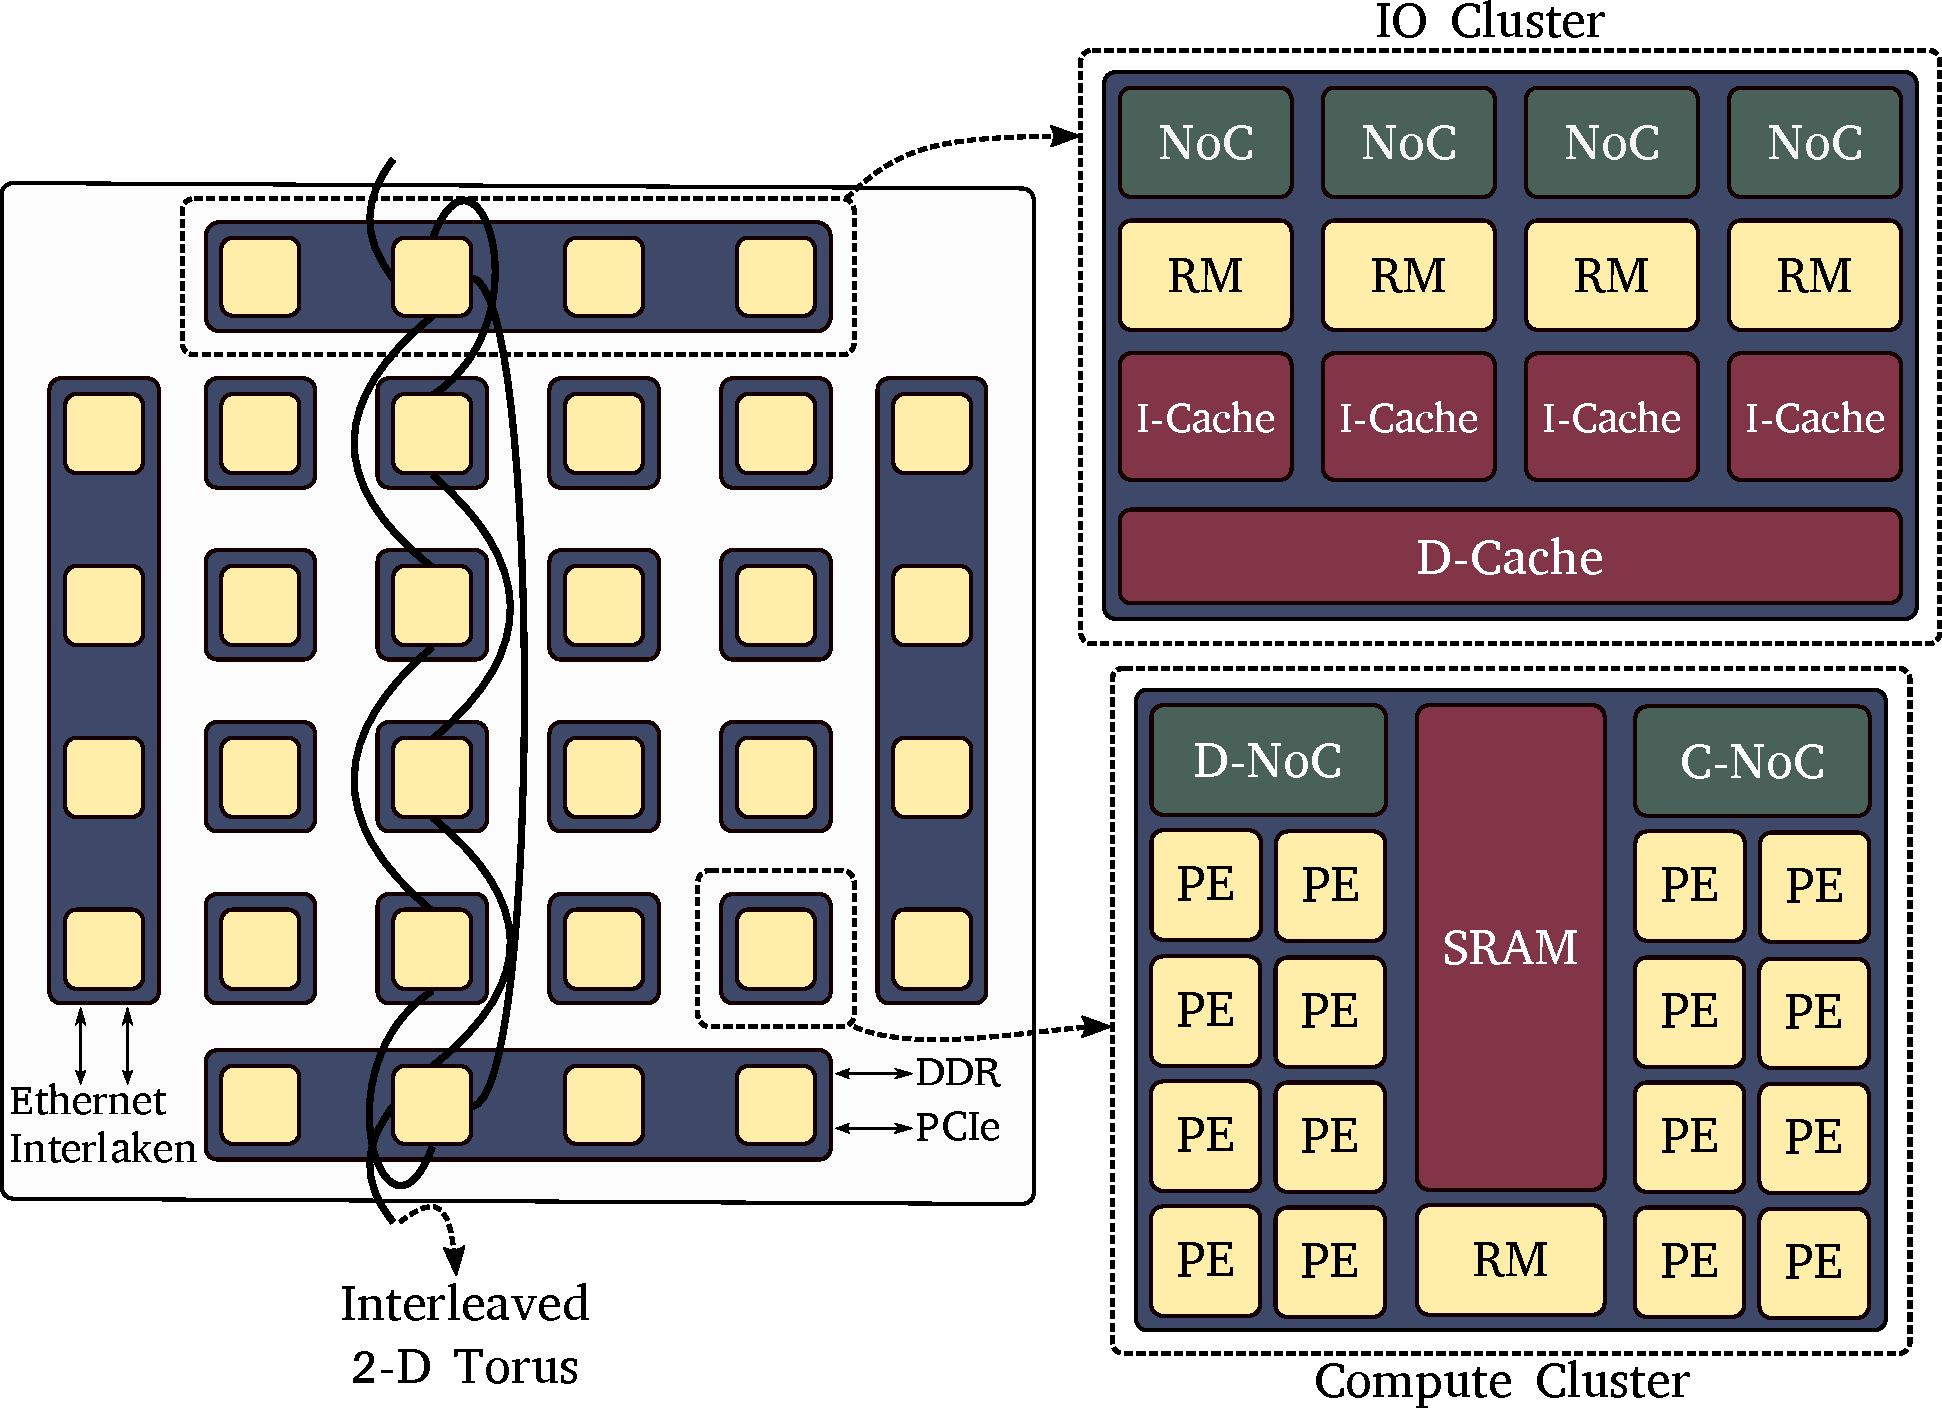
\includegraphics[width=0.80\linewidth]{arch-mppa}
			\caption{\mppa Architecture Overview.}
			\label{fig:mppa}
	\end{figure}

